\chapter{A \textit{ISA RISC-V}}\label{CapISA}

%\resumodocapitulo{Resumo opcional}

\section{Visão Geral da Arquitetura}
{
    A \textit{ISA RISC-V} é uma arquitetura modular, sendo o módulo base de
    operações com inteiros mandatório em qualquer implementação. Os demais
    módulos são extensões de uso opcional. A arquitetura não suporta
    \textit{branch delay slots} e aceita instruções de tamanho variável. A
    codificação das instruções de tamanho variável é mostrada na
    Figura~\ref{fig:riscv_var_length}. As instruções presentes no módulo
    base correspondem ao mínimo necessário para emular por
    \textit{software} as demais extensões (com exceção das operações
    atômicas).
}

\begin{figure}[H]
\centering
    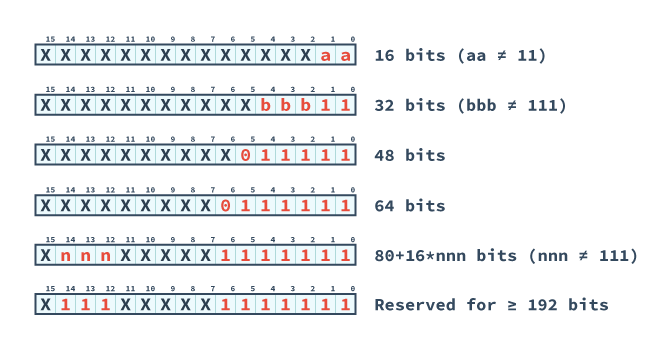
\includegraphics[width=1\linewidth]{images/RV_InstructionLength.png}
    \caption{Codificação de instruções de tamanho variável da arquitetura
                \textit{RISC-V}}\label{fig:riscv_var_length}
\end{figure}

\clearpage

{
    A nomenclatura do conjunto de instruções implementado segue a
    seguinte estrutura:
}

\begin{itemize}[leftmargin=20mm]
    \item {As letras ``RV'';}
    \item {A largura dos registradores do módulo Inteiro;}
    \item {A letra ``I'' representando a base Inteira. Caso o subconjunto
            Embarcado (\textit{Embedded}) seja implementado, substitui-se
            pela letra ``E'';}
    \item {Demais letras identificadoras de módulos opcionais.}
\end{itemize}

{
    Assim, uma implementação com registradores de 64 bits somente com o
    módulo base de Inteiros é denominado ``RV64I''.
}

\section{Módulo Inteiro}
{
    O módulo Inteiro é o módulo base da arquiterura. O \textit{design} de sua
    especificação visa reduzir o \textit{hardware} necesário para uma
    implementação mínima, bem como ser um alvo de compilação satisfatório.
}

{
    Diferente de outras arquiteturas como a \textit{ARM}, as instruções de 
    multiplicação e divisão não fazem parte do conjunto básico uam vez que
    necessitam de circuito especializado e por isso encarecem o desenvolvimento
    e produção dos processadores.
}

{
    Para sistemas embarcados com restrições mais severas de tamanho, custo,
    potência, etc o módulo base I pode ser substituído por um \textit{subset},
    o módulo E. Porém, nenhuma das demais extensões pode ser usada em conjunto
    com o módulo E.
}


\section{Extensões}
    \subsection{Extensão M}
    {
        A extensão M implementa as operações de multiplicação e divisão de
        números inteiros.
    }

    \subsection{Extensão A}
    {
        A extensão A implementa instruções de acesso atômico a memória.
        Instruções atômicas mantém a coerência da memória em sistemas
        preemptivos e paralelos.
    }

    \subsection{Extensão F}
    {
        A extensão F implementa as isntruções de ponto flutuante IEEE 754 de
        precisão simples, bem como o banco de registradores especializado para
        operações com ponto flutuante.
    }

    \subsection{Extensão D}
    {
        A extensão D implementa as instruções de ponto flutuante IEEE 754 de
        precisão dupla. Ela é um incremento à extensão F, sendo esta de
        implementação obrigatória para se poder implementar a extensão D.
    }

    \subsection{Outras Extensões}
    {
        Outras extensões são previstas na especificação da arquitetura, e.g.
        a extensão C para instruções comprimidas (16 bits).
    }

    {
        A arquitetura prevê a expansão de extensões, com alguns
        \textit{opcodes} sendo reservados para essa finalidade. Desse modo,
        instruções proprietárias e/ou customisadas podem ser adicionadas.
    }

\section{Arquitetura Privilegiada}
{
    Para a \textit{ISA RISC-V}, existem quatro níveis de privilégio de acesso,
    sendo eles o de usuário (módulo I e extensões), de máquina 
    (\textit{syscalls}) de supervisor (sistema operacional) e hipervisor
    (virtualização).
}

\section{Formatos de Instruções}
{
    As instruções da arquitetura podem ser separadas em subgrupos de acordo com
    os operadores necessários para o processador interpretá-la. A 
    Figura~\ref{fig:riscv_formats} apresenta os formatos das instruções do
    módulo I da \textit{ISA RISC-V}, e, para efeitos de comparação, a
    Figura~\ref{fig:mips_formats} mostra os formatos de instruções equivalentes
    na arquitetura MIPS32.
}

\begin{figure}[H]
\centering
    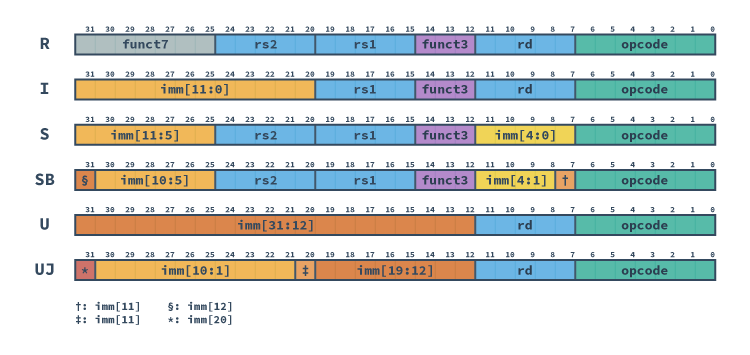
\includegraphics[width=1\linewidth]{images/RV_Formats.png}
    \caption{Formatos de Instruções da\textit{ISA RISC-V}
        }\label{fig:riscv_formats}
\end{figure}

\begin{figure}[H]
\centering
    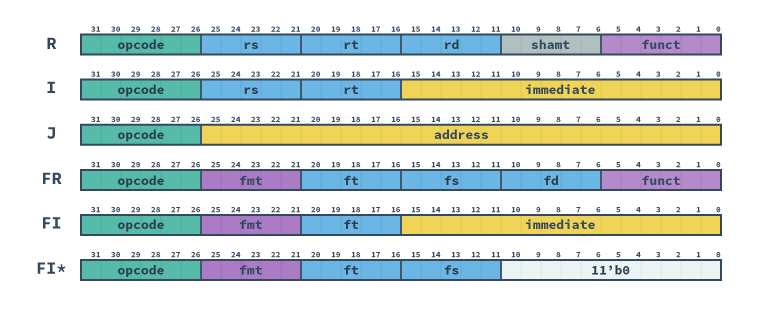
\includegraphics[width=1\linewidth]{images/MIPS_Formats.png}
    \caption{Formatos de Instruções da \textit{ISA MIPS32}
        }\label{fig:mips_formats}
\end{figure}

\section{Formatos de Imediatos}
{
    Os imediatos são operandos descritos na própria instrução em vez de estar
    contido em um registrador. Como os operandos necessitam ter a mesma largura
    que o banco de registradores, algumas regras são utilizadas para gerar os
    operandos imediatos. As figuras a seguir mostram a formação de cada tipo de
    imediato dos formatos da Figura~\ref{fig:riscv_formats}.
}

\begin{figure}[H]
\centering
    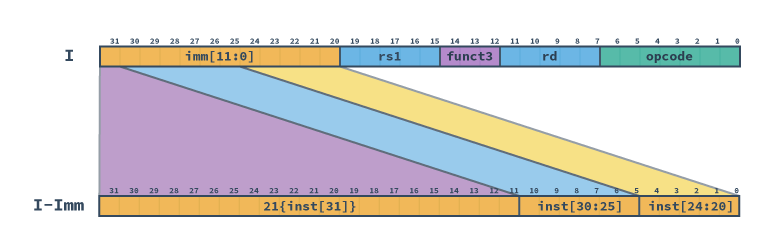
\includegraphics[width=1\linewidth]{images/RV_I_Imm.png}
    \caption{Formação do Imediato de tipo I
        }\label{fig:riscv_i_imm}
\end{figure}

\begin{figure}[H]
\centering
    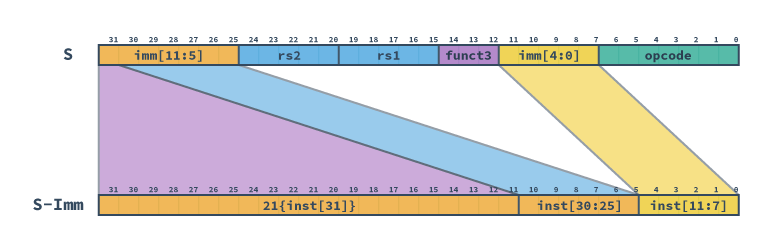
\includegraphics[width=1\linewidth]{images/RV_S_Imm.png}
    \caption{Formação do Imediato de tipo S
        }\label{fig:riscv_s_imm}
\end{figure}

\begin{figure}[H]
\centering
    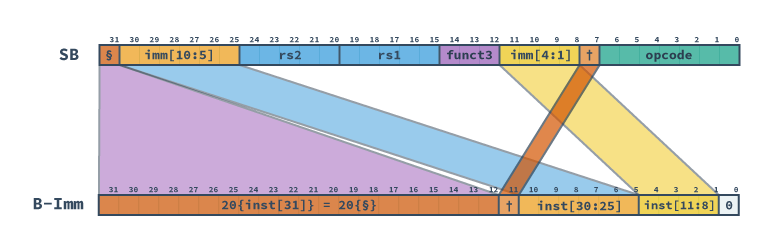
\includegraphics[width=1\linewidth]{images/RV_B_Imm.png}
    \caption{Formação do Imediato de tipo B
        }\label{fig:riscv_b_imm}
\end{figure}

\begin{figure}[H]
\centering
    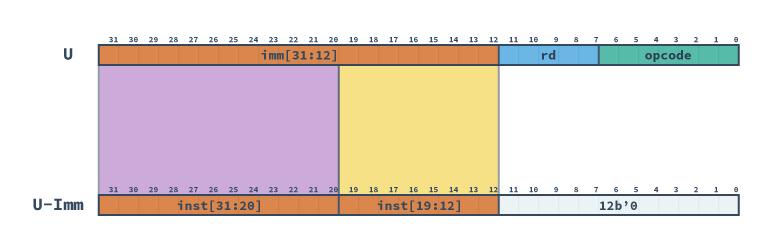
\includegraphics[width=1\linewidth]{images/RV_U_Imm.png}
    \caption{Formação do Imediato de tipo U
        }\label{fig:riscv_u_imm}
\end{figure}

\begin{figure}[H]
\centering
    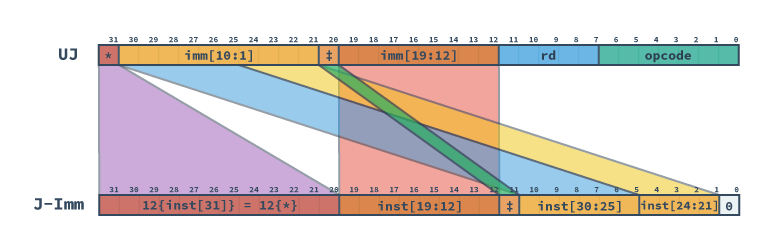
\includegraphics[width=1\linewidth]{images/RV_J_Imm.png}
    \caption{Formação do Imediato de tipo J
        }\label{fig:riscv_j_imm}
\end{figure}

{
    Para efeitos comparativos, a Figura~\ref{fig:mips_immediates} mostra a
    formação de imediatos na arquitetura MIPS32.
}

\begin{figure}[H]
\centering
    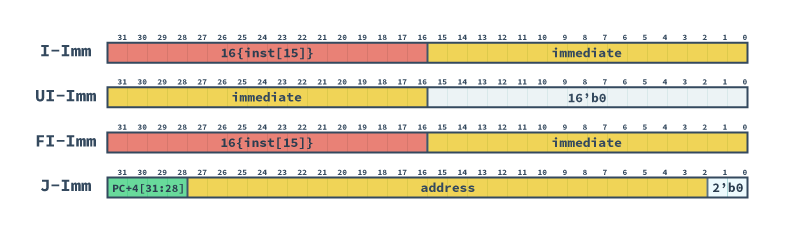
\includegraphics[width=1\linewidth]{images/MIPS_Immediates.png}
    \caption{Formatos de Imediato da \textit{ISA MIPS32}}\label{fig:mips_immediates}
\end{figure}

